\begin{figure}[h!]
\begin{center}
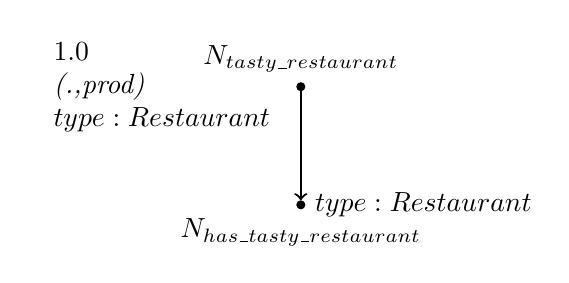
\begin{tikzpicture}[yscale=-1,
place/.style={circle,draw=black, fill=black, inner sep=0pt, 
              minimum size=1mm}]

\node[place] (1st) at (0, 0) [label=above: $N_{tasty\_restaurant}$,
                              label=left: 
             \begin{tabular}{l}
               $1.0$\\
               \textit{(.,prod)}\\
               $type : Restaurant$\\
             \end{tabular}
] {};
\node[place] (2nd) at (0, 1.5) [label=below:  $N_{has\_tasty\_restaurant}$,
label=right: 
$type : Restaurant$] {};
        
	\draw[->, thick] (1st) -- (2nd);
	
\end{tikzpicture}
\end{center}
\caption{predicate tree for tasty\_restaurant}
\label{fig:ex2.1}   
\end{figure}